\PassOptionsToPackage{unicode=true}{hyperref} % options for packages loaded elsewhere
\PassOptionsToPackage{hyphens}{url}
%
\documentclass[]{article}
\usepackage{lmodern}
\usepackage{amssymb,amsmath}
\usepackage{ifxetex,ifluatex}
\usepackage{fixltx2e} % provides \textsubscript
\ifnum 0\ifxetex 1\fi\ifluatex 1\fi=0 % if pdftex
  \usepackage[T1]{fontenc}
  \usepackage[utf8]{inputenc}
  \usepackage{textcomp} % provides euro and other symbols
\else % if luatex or xelatex
  \usepackage{unicode-math}
  \defaultfontfeatures{Ligatures=TeX,Scale=MatchLowercase}
\fi
% use upquote if available, for straight quotes in verbatim environments
\IfFileExists{upquote.sty}{\usepackage{upquote}}{}
% use microtype if available
\IfFileExists{microtype.sty}{%
\usepackage[]{microtype}
\UseMicrotypeSet[protrusion]{basicmath} % disable protrusion for tt fonts
}{}
\IfFileExists{parskip.sty}{%
\usepackage{parskip}
}{% else
\setlength{\parindent}{0pt}
\setlength{\parskip}{6pt plus 2pt minus 1pt}
}
\usepackage{hyperref}
\hypersetup{
            pdftitle={Stochastic Processes: Assignment 1},
            pdfauthor={Group 1: Javier Esteban Aragoneses, Mauricio Marcos Fajgenbaun, Danyu Zhang, Daniel Alonso},
            pdfborder={0 0 0},
            breaklinks=true}
\urlstyle{same}  % don't use monospace font for urls
\usepackage[margin=1in]{geometry}
\usepackage{color}
\usepackage{fancyvrb}
\newcommand{\VerbBar}{|}
\newcommand{\VERB}{\Verb[commandchars=\\\{\}]}
\DefineVerbatimEnvironment{Highlighting}{Verbatim}{commandchars=\\\{\}}
% Add ',fontsize=\small' for more characters per line
\usepackage{framed}
\definecolor{shadecolor}{RGB}{248,248,248}
\newenvironment{Shaded}{\begin{snugshade}}{\end{snugshade}}
\newcommand{\AlertTok}[1]{\textcolor[rgb]{0.94,0.16,0.16}{#1}}
\newcommand{\AnnotationTok}[1]{\textcolor[rgb]{0.56,0.35,0.01}{\textbf{\textit{#1}}}}
\newcommand{\AttributeTok}[1]{\textcolor[rgb]{0.77,0.63,0.00}{#1}}
\newcommand{\BaseNTok}[1]{\textcolor[rgb]{0.00,0.00,0.81}{#1}}
\newcommand{\BuiltInTok}[1]{#1}
\newcommand{\CharTok}[1]{\textcolor[rgb]{0.31,0.60,0.02}{#1}}
\newcommand{\CommentTok}[1]{\textcolor[rgb]{0.56,0.35,0.01}{\textit{#1}}}
\newcommand{\CommentVarTok}[1]{\textcolor[rgb]{0.56,0.35,0.01}{\textbf{\textit{#1}}}}
\newcommand{\ConstantTok}[1]{\textcolor[rgb]{0.00,0.00,0.00}{#1}}
\newcommand{\ControlFlowTok}[1]{\textcolor[rgb]{0.13,0.29,0.53}{\textbf{#1}}}
\newcommand{\DataTypeTok}[1]{\textcolor[rgb]{0.13,0.29,0.53}{#1}}
\newcommand{\DecValTok}[1]{\textcolor[rgb]{0.00,0.00,0.81}{#1}}
\newcommand{\DocumentationTok}[1]{\textcolor[rgb]{0.56,0.35,0.01}{\textbf{\textit{#1}}}}
\newcommand{\ErrorTok}[1]{\textcolor[rgb]{0.64,0.00,0.00}{\textbf{#1}}}
\newcommand{\ExtensionTok}[1]{#1}
\newcommand{\FloatTok}[1]{\textcolor[rgb]{0.00,0.00,0.81}{#1}}
\newcommand{\FunctionTok}[1]{\textcolor[rgb]{0.00,0.00,0.00}{#1}}
\newcommand{\ImportTok}[1]{#1}
\newcommand{\InformationTok}[1]{\textcolor[rgb]{0.56,0.35,0.01}{\textbf{\textit{#1}}}}
\newcommand{\KeywordTok}[1]{\textcolor[rgb]{0.13,0.29,0.53}{\textbf{#1}}}
\newcommand{\NormalTok}[1]{#1}
\newcommand{\OperatorTok}[1]{\textcolor[rgb]{0.81,0.36,0.00}{\textbf{#1}}}
\newcommand{\OtherTok}[1]{\textcolor[rgb]{0.56,0.35,0.01}{#1}}
\newcommand{\PreprocessorTok}[1]{\textcolor[rgb]{0.56,0.35,0.01}{\textit{#1}}}
\newcommand{\RegionMarkerTok}[1]{#1}
\newcommand{\SpecialCharTok}[1]{\textcolor[rgb]{0.00,0.00,0.00}{#1}}
\newcommand{\SpecialStringTok}[1]{\textcolor[rgb]{0.31,0.60,0.02}{#1}}
\newcommand{\StringTok}[1]{\textcolor[rgb]{0.31,0.60,0.02}{#1}}
\newcommand{\VariableTok}[1]{\textcolor[rgb]{0.00,0.00,0.00}{#1}}
\newcommand{\VerbatimStringTok}[1]{\textcolor[rgb]{0.31,0.60,0.02}{#1}}
\newcommand{\WarningTok}[1]{\textcolor[rgb]{0.56,0.35,0.01}{\textbf{\textit{#1}}}}
\usepackage{graphicx,grffile}
\makeatletter
\def\maxwidth{\ifdim\Gin@nat@width>\linewidth\linewidth\else\Gin@nat@width\fi}
\def\maxheight{\ifdim\Gin@nat@height>\textheight\textheight\else\Gin@nat@height\fi}
\makeatother
% Scale images if necessary, so that they will not overflow the page
% margins by default, and it is still possible to overwrite the defaults
% using explicit options in \includegraphics[width, height, ...]{}
\setkeys{Gin}{width=\maxwidth,height=\maxheight,keepaspectratio}
\setlength{\emergencystretch}{3em}  % prevent overfull lines
\providecommand{\tightlist}{%
  \setlength{\itemsep}{0pt}\setlength{\parskip}{0pt}}
\setcounter{secnumdepth}{0}
% Redefines (sub)paragraphs to behave more like sections
\ifx\paragraph\undefined\else
\let\oldparagraph\paragraph
\renewcommand{\paragraph}[1]{\oldparagraph{#1}\mbox{}}
\fi
\ifx\subparagraph\undefined\else
\let\oldsubparagraph\subparagraph
\renewcommand{\subparagraph}[1]{\oldsubparagraph{#1}\mbox{}}
\fi

% set default figure placement to htbp
\makeatletter
\def\fps@figure{htbp}
\makeatother


\title{Stochastic Processes: Assignment 1}
\author{Group 1: Javier Esteban Aragoneses, Mauricio Marcos Fajgenbaun, Danyu
Zhang, Daniel Alonso}
\date{January 10th, 2020}

\begin{document}
\maketitle

\hypertarget{problem-1}{%
\section{Problem 1}\label{problem-1}}

This is our implementation of the decoding algorithm, it is implemented
using python. Every single step is explained during the code with its
corresponding block or line(s) of code.

\begin{Shaded}
\begin{Highlighting}[]
\CommentTok{# importing libraries}
\ImportTok{import}\NormalTok{ numpy }\ImportTok{as}\NormalTok{ np}
\ImportTok{from}\NormalTok{ copy }\ImportTok{import}\NormalTok{ deepcopy}
\ImportTok{import}\NormalTok{ pandas }\ImportTok{as}\NormalTok{ pd}
\ImportTok{import}\NormalTok{ matplotlib.pyplot }\ImportTok{as}\NormalTok{ plt}
\ImportTok{from}\NormalTok{ nltk.corpus }\ImportTok{import}\NormalTok{ words}

\CommentTok{# Importing the matrix with the frequencies}
\NormalTok{freq }\OperatorTok{=}\NormalTok{  np.loadtxt(}\StringTok{'./data/Englishcharacters.txt'}\NormalTok{, usecols}\OperatorTok{=}\BuiltInTok{range}\NormalTok{(}\DecValTok{27}\NormalTok{))}

\CommentTok{# transformation function for table values}
\KeywordTok{def}\NormalTok{ transf_log(table):}
    \ControlFlowTok{return}\NormalTok{ np.log(table }\OperatorTok{+} \DecValTok{1}\NormalTok{)}

\CommentTok{# applying the transformation function}
\NormalTok{freq }\OperatorTok{=}\NormalTok{ transf_log(freq)}

\CommentTok{# importing the messages and only selecting the }
\CommentTok{# message with index 0, as this is the one corresponding}
\CommentTok{# to group 1}
\ControlFlowTok{with} \BuiltInTok{open}\NormalTok{(}\StringTok{'./data/messages.txt'}\NormalTok{) }\ImportTok{as}\NormalTok{ f:}
\NormalTok{    message }\OperatorTok{=}\NormalTok{ f.readlines()[}\DecValTok{0}\NormalTok{].replace(}\StringTok{'}\CharTok{\textbackslash{}n}\StringTok{'}\NormalTok{,}\StringTok{''}\NormalTok{)}

\CommentTok{# decode function}
\KeywordTok{def}\NormalTok{ decode(message, freqs, iters, check_words}\OperatorTok{=}\VariableTok{True}\NormalTok{):}
    \CommentTok{"""}
\CommentTok{    Function to decode a message enconded }
\CommentTok{    using a substitution cipher utilizing the}
\CommentTok{    Metropolis-Hastings algorithm.}

\CommentTok{    Params:}
\CommentTok{    message =     string to decode}
\CommentTok{    freqs =       frequency table for transitions of letters}
\CommentTok{                  to input}
\CommentTok{    iters =       amount of iterations to perform}
\CommentTok{    check_words = if true the loop will be broken if 5 words}
\CommentTok{                  in the message are found to be in the english}
\CommentTok{                  language corpus, if false then the function will}
\CommentTok{                  print the message after the condition where}
\CommentTok{                  min(a(f*,f), 1) > random uniformly distributed number between}
\CommentTok{                  0 and 1}
\CommentTok{    """}
    \CommentTok{# dictionary to organize the iterations}
    \CommentTok{# the score and the result of the attempt}
    \CommentTok{# to decode the message corresponding to that}
    \CommentTok{# iteration}
\NormalTok{    msg_iters }\OperatorTok{=}\NormalTok{ \{\}}

    \CommentTok{# defining the identity function}
    \CommentTok{# all letters to be used excluding spaces}
\NormalTok{    letters }\OperatorTok{=}\NormalTok{ [}\StringTok{"a"}\NormalTok{, }\StringTok{"b"}\NormalTok{, }\StringTok{"c"}\NormalTok{, }\StringTok{"d"}\NormalTok{,}
                \StringTok{"e"}\NormalTok{, }\StringTok{"f"}\NormalTok{, }\StringTok{"g"}\NormalTok{, }\StringTok{"h"}\NormalTok{, }
                \StringTok{"i"}\NormalTok{, }\StringTok{"j"}\NormalTok{, }\StringTok{"k"}\NormalTok{, }\StringTok{"l"}\NormalTok{, }
                \StringTok{"m"}\NormalTok{, }\StringTok{"n"}\NormalTok{, }\StringTok{"o"}\NormalTok{, }\StringTok{"p"}\NormalTok{, }
                \StringTok{"q"}\NormalTok{, }\StringTok{"r"}\NormalTok{, }\StringTok{"s"}\NormalTok{, }\StringTok{"t"}\NormalTok{, }
                \StringTok{"u"}\NormalTok{, }\StringTok{"v"}\NormalTok{, }\StringTok{"w"}\NormalTok{, }\StringTok{"x"}\NormalTok{, }
                \StringTok{"y"}\NormalTok{, }\StringTok{"z"}\NormalTok{]}
    \CommentTok{# creating a copy of the original letters}
    \CommentTok{# to use as key for the dictionaries}
\NormalTok{    init_letters }\OperatorTok{=}\NormalTok{ deepcopy(letters)}
    \CommentTok{# creating a dictionary with init_letters as keys}
    \CommentTok{# and letters as values}
\NormalTok{    cd }\OperatorTok{=}\NormalTok{ \{l:d }\ControlFlowTok{for}\NormalTok{ l,d }\KeywordTok{in} \BuiltInTok{zip}\NormalTok{(init_letters,letters)\}}
    \CommentTok{# every time we update with \{' ':' '\} we add the space}
    \CommentTok{# to the dictionary}
\NormalTok{    cd.update(\{}\StringTok{' '}\NormalTok{:}\StringTok{' '}\NormalTok{\})}
    \CommentTok{# define a function that just uses the previous}
    \CommentTok{# dictionary to seek the letters}
    \KeywordTok{def}\NormalTok{ f(c):}
        \ControlFlowTok{return}\NormalTok{ cd[c]}
    
    \CommentTok{# this dictionary and subsequent function maps each letter}
    \CommentTok{# to a column/row in the freq matrix, ex: 'a':0, 'b':1 }
\NormalTok{    fvals }\OperatorTok{=}\NormalTok{ np.array([x }\ControlFlowTok{for}\NormalTok{ x }\KeywordTok{in} \BuiltInTok{range}\NormalTok{(}\BuiltInTok{len}\NormalTok{(letters))])}
\NormalTok{    cd_map }\OperatorTok{=}\NormalTok{ \{l:v }\ControlFlowTok{for}\NormalTok{ l,v }\KeywordTok{in} \BuiltInTok{zip}\NormalTok{(letters,fvals)\}}
\NormalTok{    cd_map.update(\{}\StringTok{' '}\NormalTok{:}\DecValTok{26}\NormalTok{\})}
    \KeywordTok{def}\NormalTok{ f_map(c):}
        \ControlFlowTok{return}\NormalTok{ cd_map[c]}

    \CommentTok{# score function uses sum of logs}
    \KeywordTok{def}\NormalTok{ score(fun):}
\NormalTok{        p }\OperatorTok{=} \DecValTok{0}
        \ControlFlowTok{for}\NormalTok{ i }\KeywordTok{in} \BuiltInTok{range}\NormalTok{(}\DecValTok{1}\NormalTok{,}\BuiltInTok{len}\NormalTok{(msg)):}
\NormalTok{            p }\OperatorTok{=}\NormalTok{ p }\OperatorTok{+}\NormalTok{ freqs[f_map(fun(msg[i}\DecValTok{-1}\NormalTok{])),f_map(fun(msg[i]))]}
        \ControlFlowTok{return}\NormalTok{ p}
    
    \CommentTok{# converting the message to a list in order to}
    \CommentTok{# go through the letters in pairs}
\NormalTok{    msg }\OperatorTok{=} \BuiltInTok{list}\NormalTok{(message)}

    \CommentTok{# letters list, this one shall be modified}
    \CommentTok{# every time the score passes the test}
\NormalTok{    letters_n }\OperatorTok{=}\NormalTok{ deepcopy(letters)}

    \CommentTok{# loop iters amount of times}
    \ControlFlowTok{for}\NormalTok{ i }\KeywordTok{in} \BuiltInTok{range}\NormalTok{(iters):}
        \CommentTok{# randomly choose 2 numbers and replace the 2 chosen }
        \CommentTok{# vals in a copy of letters}
\NormalTok{        ch1 }\OperatorTok{=}\NormalTok{ np.random.randint(}\DecValTok{0}\NormalTok{,}\BuiltInTok{len}\NormalTok{(letters))}
\NormalTok{        ch2 }\OperatorTok{=}\NormalTok{ np.random.randint(}\DecValTok{0}\NormalTok{,}\BuiltInTok{len}\NormalTok{(letters))}
\NormalTok{        plc1 }\OperatorTok{=}\NormalTok{ deepcopy(letters_n[ch1])}
\NormalTok{        plc2 }\OperatorTok{=}\NormalTok{ deepcopy(letters_n[ch2])}
\NormalTok{        letters_n[ch1] }\OperatorTok{=}\NormalTok{ plc2}
\NormalTok{        letters_n[ch2] }\OperatorTok{=}\NormalTok{ plc1}

        \CommentTok{# create the dictionary for the f* function}
\NormalTok{        cd_n }\OperatorTok{=}\NormalTok{ \{l:v }\ControlFlowTok{for}\NormalTok{ l,v }\KeywordTok{in} \BuiltInTok{zip}\NormalTok{(init_letters,letters_n)\}}
        \CommentTok{# add the space to it after scramble}
\NormalTok{        cd_n.update(\{}\StringTok{' '}\NormalTok{:}\StringTok{' '}\NormalTok{\})}
        \CommentTok{# f* definition}
        \KeywordTok{def}\NormalTok{ f_n(c):}
            \ControlFlowTok{return}\NormalTok{ cd_n[c]}
    
        \CommentTok{# calculating the score for each function and its ratio}
\NormalTok{        scr_f }\OperatorTok{=}\NormalTok{ score(f)}
\NormalTok{        scr_fn }\OperatorTok{=}\NormalTok{ score(f_n)}
\NormalTok{        a }\OperatorTok{=}\NormalTok{ np.exp(scr_fn }\OperatorTok{-}\NormalTok{ scr_f)}
        \CommentTok{# test if a random number is lower than min(a, 1)}
\NormalTok{        cond }\OperatorTok{=}\NormalTok{ np.random.rand() }\OperatorTok{<} \BuiltInTok{min}\NormalTok{(a,}\DecValTok{1}\NormalTok{)}
        \CommentTok{# if condition is true}
        \ControlFlowTok{if}\NormalTok{ cond:}
            \CommentTok{# replacing the letters list with the one from f*}
\NormalTok{            letters }\OperatorTok{=}\NormalTok{ deepcopy(letters_n)}
            \CommentTok{# updating the dictionary with the new letters list after replacing}
\NormalTok{            cd }\OperatorTok{=}\NormalTok{ \{l:v }\ControlFlowTok{for}\NormalTok{ l,v }\KeywordTok{in} \BuiltInTok{zip}\NormalTok{(init_letters,letters)\}}
\NormalTok{            cd.update(\{}\StringTok{' '}\NormalTok{:}\StringTok{' '}\NormalTok{\})}
            \CommentTok{# f re-definition}
            \KeywordTok{def}\NormalTok{ f(c):}
                \ControlFlowTok{return}\NormalTok{ cd[c]}
            \CommentTok{# replacing the letters in the message using }
            \CommentTok{# the new f replaced by f*}
            \ControlFlowTok{for}\NormalTok{ k }\KeywordTok{in} \BuiltInTok{range}\NormalTok{(}\BuiltInTok{len}\NormalTok{(msg)):}
\NormalTok{                msg[k] }\OperatorTok{=}\NormalTok{ f(msg[k])}
            \CommentTok{# adding score and joining the message to the dictionary}
            \CommentTok{# to then transform into a dataframe}
\NormalTok{            msg_iters[i] }\OperatorTok{=}\NormalTok{ (a,}\StringTok{''}\NormalTok{.join([x }\ControlFlowTok{for}\NormalTok{ x }\KeywordTok{in}\NormalTok{ msg]))}

            \CommentTok{# we separate the message by words}
\NormalTok{            msg_list }\OperatorTok{=}\NormalTok{ msg_iters[i][}\DecValTok{1}\NormalTok{].split(}\StringTok{' '}\NormalTok{)}
            \CommentTok{# we test 5 random words to see if they are actually words }
            \CommentTok{# present in the word corpus}
\NormalTok{            conds }\OperatorTok{=}\NormalTok{ [np.random.choice(msg_list) }\KeywordTok{in}\NormalTok{ words.words() }\ControlFlowTok{for}\NormalTok{ x }\KeywordTok{in} \BuiltInTok{range}\NormalTok{(}\DecValTok{5}\NormalTok{)]}
            \CommentTok{# if check words == True}
            \ControlFlowTok{if}\NormalTok{ check_words }\OperatorTok{==} \VariableTok{True}\NormalTok{:}
                \CommentTok{# we break the loop if the 5 true words are found}
                \ControlFlowTok{if} \VariableTok{False} \KeywordTok{not} \KeywordTok{in}\NormalTok{ conds:}
                    \BuiltInTok{print}\NormalTok{(}\StringTok{'Cipher used:}\CharTok{\textbackslash{}n}\StringTok{'}\NormalTok{)}
                    \BuiltInTok{print}\NormalTok{(}\SpecialStringTok{f'}\SpecialCharTok{\{cd\}}\SpecialStringTok{'}\NormalTok{)}
                    \BuiltInTok{print}\NormalTok{(}\SpecialStringTok{f'}\CharTok{\textbackslash{}n}\SpecialStringTok{found at iteration: }\SpecialCharTok{\{i\}}\CharTok{\textbackslash{}n}\SpecialStringTok{Message (may contain wrong letters):'}\NormalTok{)}
                    \ControlFlowTok{return}\NormalTok{ msg_iters[i]}
            \CommentTok{# otherwise}
            \ControlFlowTok{else}\NormalTok{:}
                \CommentTok{# we print the iteration number and message only }
                \CommentTok{# when the cipher changes}
                \BuiltInTok{print}\NormalTok{(}\SpecialStringTok{f'iteration #}\SpecialCharTok{\{i\}}\SpecialStringTok{:}\CharTok{\textbackslash{}n}\SpecialStringTok{'}\NormalTok{)}
                \BuiltInTok{print}\NormalTok{(}\SpecialStringTok{f'}\SpecialCharTok{\{}\NormalTok{msg_iters[i][}\DecValTok{1}\NormalTok{]}\SpecialCharTok{\}}\CharTok{\textbackslash{}n}\SpecialStringTok{'}\NormalTok{)}
        \CommentTok{# if condition is false}
        \ControlFlowTok{else}\NormalTok{:}
            \CommentTok{# resetting the letters after a failed score comparison}
\NormalTok{            letters_n }\OperatorTok{=}\NormalTok{ deepcopy(letters)}
            \CommentTok{# apply the f function to the message instead}
            \ControlFlowTok{for}\NormalTok{ k }\KeywordTok{in} \BuiltInTok{range}\NormalTok{(}\BuiltInTok{len}\NormalTok{(msg)):}
\NormalTok{                msg[k] }\OperatorTok{=}\NormalTok{ f(msg[k])}
        
        \CommentTok{# reset the message}
\NormalTok{        msg }\OperatorTok{=} \BuiltInTok{list}\NormalTok{(message)}

    \CommentTok{# put the information in a dataframe, iters, score and the messages}
\NormalTok{    df }\OperatorTok{=}\NormalTok{ \{}\StringTok{'iter'}\NormalTok{:[it }\ControlFlowTok{for}\NormalTok{ it }\KeywordTok{in}\NormalTok{ msg_iters.keys()],}
          \StringTok{'score'}\NormalTok{:[msg[}\DecValTok{0}\NormalTok{] }\ControlFlowTok{for}\NormalTok{ msg }\KeywordTok{in}\NormalTok{ msg_iters.values()],}
          \StringTok{'msg'}\NormalTok{:[msg[}\DecValTok{1}\NormalTok{] }\ControlFlowTok{for}\NormalTok{ msg }\KeywordTok{in}\NormalTok{ msg_iters.values()]\}}
    \CommentTok{# return the dataframe in case the loop was never broken}
    \ControlFlowTok{return}\NormalTok{ pd.DataFrame(df)}
\end{Highlighting}
\end{Shaded}

Our function seems to oscillate between a nearly fully decoded message
where b is mapped to p and the opposite (when it's allowed to run
without a break)

As a result we obtain the following decoded message (either decoding by
hand the last few wrong letters in the cipher):

``\emph{a day after britain became the first western country to
authorize a coronavirus vaccine british and american officials bickered
over which governments drug approval process was better leading
scientists to warn that the debate could undermine public faith vaccine
nationalism has no place in covid or other public health matters of
global significance said a scientific adviser to the british government
science has always been the exit strategy from this horrendous pandemic
several top british lawmakers have also incorrectly cast the countrys
split with the european union as the reason it authorized a vaccine
first in fact britain remains under the blocs regulatory umbrella and
was able to move more quickly because of an old law enabling it to make
its own determinations in public health emergencies}''

The message is fully decrypted after a variable number of iterations,
sometimes it takes 3,000 iters but other tiems it might take 60,000
iters.

\newpage

\hypertarget{problem-2}{%
\section{Problem 2}\label{problem-2}}

\hypertarget{a}{%
\section{(a)}\label{a}}

Let \textbf{\(N(t)\)} be the number of cars arriving at a parking lot by
time \textbf{\(t\)}, according to the proposed scenario, we can model
\textbf{\(N(t)\)} as a non-homogenous Poisson process. Such process has
almost the same process as any other Poisson process, however, its rate
is a function of time.

\(N(t), t \in [0, \infty)\) is the non-homogenous Poisson process with
rate \(\lambda (t)\) where:

\begin{itemize}
\tightlist
\item
  \(N(0) = 0\)
\item
  \(N(t)\) has independent increments
\item
  for any \(t \in [0, \infty)\), we have:

  \begin{itemize}
  \tightlist
  \item
    \(P(N(t + \Delta) - N(t) = 0) = 1 - \lambda (t) \Delta + o(\Delta)\)
  \item
    \(P(N(t + \Delta) - N(t) = 1) = \lambda (t) \Delta + o(\Delta)\)
  \item
    \(P(N(t + \Delta) - N(t) \geq 2) = o(\Delta)\)
  \end{itemize}
\end{itemize}

We define 8:00 as \(t=0\) with the following integrable function and
each unit of \(t\) equals to 1 hour:

\(\lambda (t) = \begin{cases} 100 & 0 \leq t \leq \frac{1}{2} \\ 600t - 200 & \frac{1}{2} < t \leq \frac{3}{4} \\ 400t - 50 & \frac{3}{4} < t \leq 1 \\ -500t + 850 & 1 < t \leq 1.5 \\ \end{cases}\)

We define, for all \(t > 0, N_t\) has a poisson distribution with mean:

\(E(N_t) = \int_{0}^t \lambda x\,dx\)

So,

\(E[N(t)] = \begin{cases} \int_{0}^t 100\,dt = 100t & 0 \leq t \leq \frac{1}{2} \\ \int_{\frac{1}{2}}^t 600t - 200 \,dt + 50 = 300(t^2 - \frac{1}{4}) - 200(t - \frac{1}{2}) + 50 & \frac{1}{2} < t \leq \frac{3}{4} \\ \int_{\frac{3}{4}}^t 400t - 50 \,dt + 93.75 = 25(8t^2 - 2t - 3) + 93.75 & \frac{3}{4} < t \leq 1 \\ \int_{1}^t -500t + 850\,dt + 168.75 = -50(5t^2 - 17t + 12) + 168.75 & 1 < t \leq 1.5 \end{cases}\)

Given that there is a limit of 150 vehicles:

\(E[N(t)] = \begin{cases} 100t & 0 \leq t \leq \frac{1}{2} \\ 300(t^2 - \frac{1}{4}) - 200(t - \frac{1}{2}) + 50 & \frac{1}{2} < t \leq \frac{3}{4} \\ 25(8t^2 - 2t - 3) + 93.75 & \frac{3}{4} < t < 0.94468 \\ 150 & t \geq 0.94468 \end{cases}\)

\hypertarget{b}{%
\section{(b)}\label{b}}

We are asked the time in which, with a probability of 0.8, the number of
vehicles in the parking lot is strictly less than 150. This way, we have
a place in the parking. This is the same as saying that we want 0.8 to
be the probability of having 149 or less cars in the parking. The
function \emph{ppois} in R, calculates (through the number of events and
lambda) the probability of those events or less happening in the
process. As we do have the probability, but are interested in finding
lambda, what we do is try different values of lambda, until we get a
probability equal to 0.8.

First, we try going unit by unit. When we know that it is between 139
and 140, we do the same but going in intervals of size 0.1. That is
trying with values: 139.1, 139.2, and more.

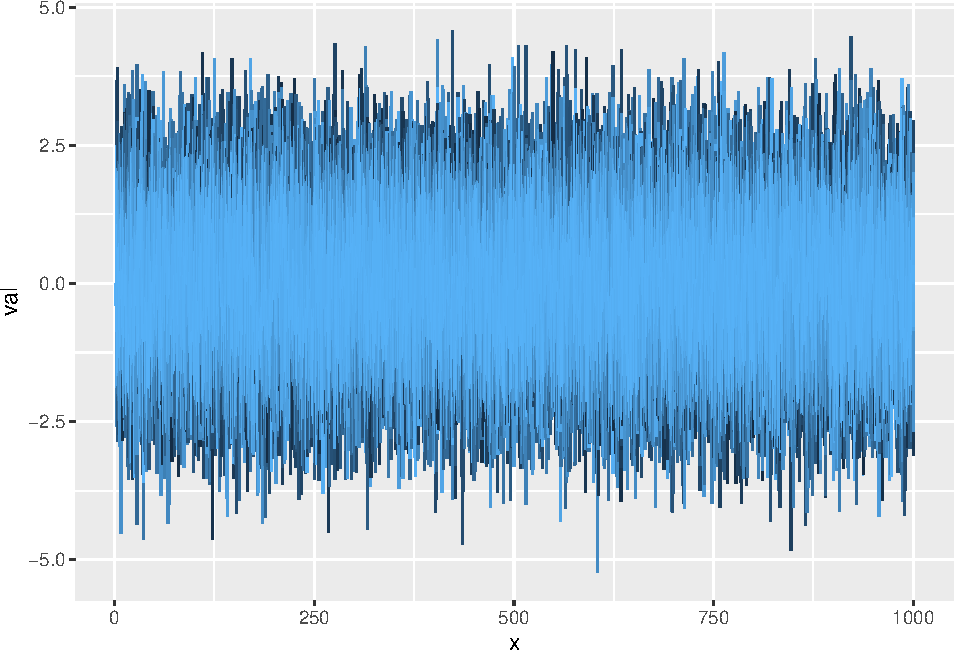
\includegraphics{./figures/unnamed-chunk-3-1.pdf}
\includegraphics{./figures/unnamed-chunk-3-2.pdf}

Once we get lambda, with the expected value of events that we previously
calculated, we tried calculating the times in the third interval.

As the time tested fits within the interval we are looking for, we know
that it is the right one.

For example, if we use the first interval, the time calculated does not
fit into its definition, and it would have been an error to consider
this.

After testing the different \(\lambda (t)\) we obtain the following:

\(\lambda (t) \approx 139.6\) and \(t \approx 0.91232\)

Finally, we transform the result to a time format (as it is currently a
decimal number representing hours) \(t = 0.91232\) hours correspond
approximately to 8:54 AM.

\newpage

\hypertarget{c}{%
\section{(c)}\label{c}}

The following function simulates a non-homogenous poisson process from a
homogenous poisson process:

\begin{Shaded}
\begin{Highlighting}[]
\NormalTok{non_hom_poisson <-}\StringTok{ }\ControlFlowTok{function}\NormalTok{(fun,l,a,b,}\DataTypeTok{start=}\DecValTok{0}\NormalTok{) \{}
    \CommentTok{# This function generates a non-homogenous poisson }
    \CommentTok{# process from a homogenous poisson process}
    \CommentTok{# PARAMS:}
    \CommentTok{# fun:   if the non-homogenous poisson process has}
    \CommentTok{#        multiple functions per time subinterval}
    \CommentTok{#        this parameters represents such function}
    \CommentTok{# l:     lambda for the homogenous poisson process}
    \CommentTok{# a:     lower bound for the time subinterval}
    \CommentTok{# b:     upper bound for the time subinterval}
    \CommentTok{# start: this parameter is used to keep track of }
    \CommentTok{#        the process count.}
    
    \CommentTok{# We generate the homogenous poisson process }
    \CommentTok{# arrival times}
\NormalTok{    val <-}\StringTok{ }\KeywordTok{rpois}\NormalTok{(}\DecValTok{1}\NormalTok{,l}\OperatorTok{*}\NormalTok{(b}\OperatorTok{-}\NormalTok{a))}
\NormalTok{    intervals <-}\StringTok{ }\NormalTok{(b}\OperatorTok{-}\NormalTok{a) }\OperatorTok{*}\StringTok{ }\KeywordTok{sort}\NormalTok{(}\KeywordTok{runif}\NormalTok{(val)) }\OperatorTok{+}\StringTok{ }\NormalTok{a}

    \CommentTok{# Non-homogenous poisson process}
\NormalTok{    evs <-}\StringTok{ }\KeywordTok{length}\NormalTok{(intervals) }\CommentTok{# lenght of arrival times }
\NormalTok{    nh_val <-}\StringTok{ }\DecValTok{0} \OperatorTok{+}\StringTok{ }\NormalTok{start }\CommentTok{# start of the event count}
\NormalTok{    nh_intervals <-}\StringTok{ }\KeywordTok{c}\NormalTok{() }\CommentTok{# arrival times for the NHPP}
    \ControlFlowTok{for}\NormalTok{ (i }\ControlFlowTok{in} \DecValTok{1}\OperatorTok{:}\NormalTok{evs) \{}
        \ControlFlowTok{if}\NormalTok{ (}\KeywordTok{runif}\NormalTok{(}\DecValTok{1}\NormalTok{) }\OperatorTok{<}\StringTok{ }\KeywordTok{fun}\NormalTok{(intervals[i])}\OperatorTok{/}\NormalTok{l) \{ }
            \CommentTok{# only including intervals from the HPP which}
            \CommentTok{# match with fun(intervals[i])/l probability}
\NormalTok{            nh_intervals <-}\StringTok{ }\KeywordTok{c}\NormalTok{(nh_intervals, intervals[i]) }
\NormalTok{            nh_val <-}\StringTok{ }\NormalTok{nh_val}\OperatorTok{+}\DecValTok{1} \CommentTok{# adding one to the event count}
\NormalTok{        \}}
\NormalTok{    \}}
\NormalTok{    nh_events <-}\StringTok{ }\KeywordTok{seq}\NormalTok{(}\DecValTok{1}\OperatorTok{+}\NormalTok{start,nh_val,}\DecValTok{1}\NormalTok{) }\CommentTok{# events since the previous group}
    \KeywordTok{return}\NormalTok{(}\KeywordTok{list}\NormalTok{(}\DataTypeTok{arrival_times=}\NormalTok{nh_intervals, }\DataTypeTok{events=}\NormalTok{nh_events))}
\NormalTok{\}}
\end{Highlighting}
\end{Shaded}

\newpage

The following code iterates over \emph{iters} amount of times the
previously defined non-homogenous poisson process with the given
function defining \(\lambda\) dependent on a parameter \(t\)
(\(\lambda (t)\)).

\begin{Shaded}
\begin{Highlighting}[]
\NormalTok{simulation <-}\StringTok{ }\ControlFlowTok{function}\NormalTok{(iters, functions, lambdas, ints) \{}
    \CommentTok{# This function simulates from the NHPP}
    \CommentTok{# iters:     number of iterations to plot and add to the list of}
    \CommentTok{#            dataframes}
    \CommentTok{# functions: list of functions corresponding to the lambda function}
    \CommentTok{# lambdas:   list of lambdas for each subinterval}
    \CommentTok{# ints:      lists of vectors of 2 elements each containing the intervals}
    \CommentTok{#            that correspond to each element of lambdas and functions lists}
\NormalTok{    p <-}\StringTok{ }\KeywordTok{list}\NormalTok{()}
    \ControlFlowTok{for}\NormalTok{ (i }\ControlFlowTok{in} \DecValTok{1}\OperatorTok{:}\NormalTok{iters) \{}
\NormalTok{        maximum <-}\StringTok{ }\DecValTok{0} \CommentTok{# start for the next NHPP simulation to continue count}
\NormalTok{        arr_times <-}\StringTok{ }\KeywordTok{c}\NormalTok{() }\CommentTok{# arrival times}
\NormalTok{        events <-}\StringTok{ }\KeywordTok{c}\NormalTok{() }\CommentTok{# event counts}
        \ControlFlowTok{for}\NormalTok{ (k }\ControlFlowTok{in} \DecValTok{1}\OperatorTok{:}\DecValTok{4}\NormalTok{) \{}
\NormalTok{            int <-}\StringTok{ }\KeywordTok{non_hom_poisson}\NormalTok{(lambda_funs[[k]],lambdas[[k]],}
\NormalTok{                                   ints[[k]][}\DecValTok{1}\NormalTok{],ints[[k]][}\DecValTok{2}\NormalTok{],}
                                   \DataTypeTok{start=}\NormalTok{maximum)}
\NormalTok{            maximum <-}\StringTok{ }\KeywordTok{max}\NormalTok{(int}\OperatorTok{$}\NormalTok{events) }\CommentTok{# remembering last event count}
\NormalTok{            arr_times <-}\StringTok{ }\KeywordTok{c}\NormalTok{(arr_times, int}\OperatorTok{$}\NormalTok{arrival_times) }
\NormalTok{            events <-}\StringTok{ }\KeywordTok{c}\NormalTok{(events, int}\OperatorTok{$}\NormalTok{events)}
\NormalTok{        \}}
\NormalTok{        p[[i]] <-}\StringTok{ }\KeywordTok{data.frame}\NormalTok{(}\DataTypeTok{arrival_times=}\NormalTok{arr_times, }\DataTypeTok{events=}\NormalTok{events)}
        \CommentTok{# plots}
        \ControlFlowTok{if}\NormalTok{ (i }\OperatorTok{==}\StringTok{ }\DecValTok{1}\NormalTok{) \{}\KeywordTok{plot}\NormalTok{(arr_times, events, }\DataTypeTok{cex=}\FloatTok{0.5}\NormalTok{, }\DataTypeTok{pch=}\StringTok{'.'}\NormalTok{, }
                          \DataTypeTok{col=}\KeywordTok{randomColor}\NormalTok{(), }\DataTypeTok{xlim=}\KeywordTok{c}\NormalTok{(}\DecValTok{0}\NormalTok{,}\FloatTok{1.5}\NormalTok{), }
                          \DataTypeTok{ylim=}\KeywordTok{c}\NormalTok{(}\DecValTok{0}\NormalTok{,}\DecValTok{150}\NormalTok{))\}}
        \KeywordTok{lines}\NormalTok{(arr_times, events, }\DataTypeTok{col=}\KeywordTok{randomColor}\NormalTok{())}
\NormalTok{    \}}
    \KeywordTok{return}\NormalTok{(p)}
\NormalTok{\}}
\end{Highlighting}
\end{Shaded}

\newpage

\hypertarget{d}{%
\section{(d)}\label{d}}

Running 1000 iterations of the simulation (we included the R output
regardless because we thought it was very pretty).

\begin{Shaded}
\begin{Highlighting}[]
\NormalTok{data <-}\StringTok{ }\KeywordTok{simulation}\NormalTok{(}\DecValTok{1000}\NormalTok{, lambda_funs, lambdas, ints)}
\end{Highlighting}
\end{Shaded}

\includegraphics{./figures/unnamed-chunk-8-1.pdf}

Proving using the 1000 simulation data that our exercise 2b is correct:

\begin{verbatim}
#> [1] 0.164
\end{verbatim}

We can see that our result approaches 0.2 very closely, which is the
remaining probability (\(1-0.8 = 0.2\)).

\hypertarget{problem-3}{%
\section{Problem 3}\label{problem-3}}

\hypertarget{a-1}{%
\section{(a)}\label{a-1}}

An M/M/c queue is a stochastic process whose state space is the set \{0,
1, 2, 3, \ldots{}\} where the value corresponds to the number of
customers in the system, including any currently in service. (n.d.)

Arrivals occur at rate \(\lambda\) according to a Poisson process and
move the process from state \emph{i} to \emph{i+1}.

Service times have an exponential distribution with parameter \(\mu\).
If there are fewer than 2 jobs, some of the servers will be free. If
there are more than 2 jobs, the jobs queue in a buffer.

The buffer is of infinite size, so there is no limit on the number of
customers it can contain.

In this case, the model describes a queue with two single servers which
serves customers in the order in which they arrive. Customer arrivals
constitute a Poisson process of rate \(\lambda\).

This means that the number of customers arriving during a time period
{[}t, t+s{]} is a Poisson random variable with mean \(\lambda\), and it
is independent of the past of the arrival process. Also, the
inter-arrival times (between the arrival of one customer and the next)
are identically distributed exponential random variables with parameter
\(\lambda\) and mean \(\frac{1}{\lambda}\). In other words, the arrival
process is Markovian, and this is what the first M in M/M/2 stands for.

The second M of this process name says that the service process is
Markovian. Customer service times are exponentially distributed, with
parameter \(\mu\) and mean \(\frac{1}{\mu}\), and the service times of
different customers are mutually independent. By the memoryless property
of the exponential distribution, knowing how much service a customer has
already received gives us no information about how much more service it
requires. When a customer has been served, it departs from the queue.
Also, in time 0, there are no costumers. So we see it fullfills all the
conditions of a Markov Chain. (Ganesh 2012)

Our infinitesimal generator is the following:

\(Q = \begin{pmatrix} - \lambda & \lambda & 0 & 0 & \dots \\ \mu & - (\lambda + \mu) & \lambda & 0 & \dots \\ 0 & 2 \mu & - (2 \mu + \lambda) & \lambda & \dots \\ \vdots & \vdots & \vdots & \vdots & \ddots \end{pmatrix}\)

\hypertarget{b-1}{%
\section{(b)}\label{b-1}}

We solve the following system:

\(\begin{cases} \sum_{i = 1}^{\infty} \pi_i = 1 \\ \lambda \pi_0 = \mu \pi_1 \\ \lambda \pi_1 = 2 \mu \pi_2 \\ \vdots \\ \lambda \pi_{n-1} = 2 \mu \pi_n \\ \vdots \\ \end{cases}\)

First we have:

\(\pi_1 = \frac{\lambda \pi_0}{\mu} \\ \pi_2 = \frac{\lambda^2 \pi_0}{2 \mu^2} \\ \pi_3 = \frac{\lambda^3 \pi_0}{2^2 \mu^3} \\ \vdots \\ \pi_n = \frac{\lambda^n \pi_0}{2^{n-1} \mu^n} \\ \vdots\)

Then:

\(\sum_{i=0}^{\infty} \pi_i = \pi_0 + \frac{\lambda \pi_0}{\mu} + \frac{\lambda^2 \pi_0}{2 \mu^2} + \dots + \frac{\lambda^n \pi_0}{2^{n-1} \mu^n} + \dots = 1\)

And so factoring \(\pi_0\) we get:

\(\pi_0 (1 + \frac{\lambda}{\mu} + \frac{\lambda^2}{2 \mu^2} + \dots) = \pi_0 (1 + \sum_{i=1}^{\infty} \frac{1}{2^{i-1}} (\frac{\lambda}{\mu})^{i})\)

Then multiplying \(\frac{2}{2}\) to the summation:

\(\pi_0 (1 + \frac{2}{2} \sum_{i=1}^{\infty} \frac{1}{2^{i-1}} (\frac{\lambda}{\mu})^{i})\)

= \(\pi_0 (2 \sum_{i=0}^{\infty} (\frac{\lambda}{2 \mu})^{i} - 1)\)

Knowing that this infite sum corresponds to a geometric series:

\(\pi_0 (2 (\frac{1}{1 - \frac{\lambda}{2 \mu}}) - 1) = 1\)

\(\pi_0 = \frac{1}{2 (\frac{1}{1 - \frac{\lambda}{2 \mu}}) - 1}\)

\(\vdots\)

\(\pi_n = \frac{\lambda^n}{2^{n-1}{\mu_n} \pi_0} \frac{1}{2 (\frac{1}{1 - \frac{\lambda}{2 \mu}}) - 1}\)

finally:

\(\pi_n = \frac{1}{2^{n-1}} (\frac{\lambda}{\mu})^{n} \pi_0\)

The infinite sum converges when \(|\frac{\lambda}{2 \mu}| < 1\) in which
case the stationary distribution P exists.

We can obtain Littles formula by finding the expectation with respect to
the stationary distribution:

\(L = \sum_{n=0}^{\infty} \pi_n * n\)

Using the following sum:

\(\sum_{i=0}^{n-1} i a^i = \frac{a - na^n + (n-1)a^{n+1}}{(1-a)^2}\)

As n approaches infinity:

\(\sum_{i=0}^{\infty} i a^i = \frac{a}{(1-a)^2}\)

We get the following:

\(L = \pi_0 [1 + \sum_{n=0}^{\infty} (\frac{\lambda}{\mu})^n * \frac{n}{2^{n-1}}]\)

\(L = \pi_0 [1 + 2 \sum_{n=0}^{\infty} (\frac{\lambda}{2 \mu})^n * n]\)

\(L = \pi_0 [1 + 2 \frac{\frac{\lambda}{2 \mu}}{(1 - \frac{\lambda}{2 \mu})^2}]\)

\hypertarget{c-1}{%
\section{(c)}\label{c-1}}

Let's consider the probabilities conditioned on the number of customers
in the system that are present once our specific subject \emph{l} gets
into the system.

If there are no other customers when \emph{l} gets into the system,
there is no chance of overtaking.

\(P(N^{OV} = 0 | N^{PR} = 0) = 1\)

With \(N^{OV}\) being the number of customers that \emph{l} overtakes
and \(N^{PR}\) the number of customers present in the system (queing)
when \emph{l} gets in the system.

If \(N^{PR} = 1\), then \emph{l} can overtake only 1 customer, if the
time it takes to be served is shorter than the time it takes the other
customers to be served. Because of the memoryless property we can assert
the following:

\(P(N^{OV} = 0 | N^{PR} = 1) = \frac{\mu}{\mu + \mu} = \frac{1}{2}\)

Actually, in general:

\(P(N^{OV} = k | N^{PR} = n) = \frac{1}{n+1}\), \(n \leq c - 1\),
\(k = 0,1\)

As in this case c=2, our \emph{l} subject can' t overtake more than one
customer.

Now, if \(n \geq c\), that is, \emph{l} has to get in queue and wait to
be served. When \emph{l} gets served, there is also one more customer
getting served. Because, again, of the memoryless property.

\(P(N^{OV} = k | N^{PR} = n) = \frac{1}{c}\), \(n = c\), \(k = 0,1\)

In our case, it does not matter how many customers are in the system,
the probability of overtaking, conditioned to the number of customers
already in the system, is \(\frac{1}{2}\).

Now, using Bayes' theorem and the total probability rule, we can find
the probability of \emph{l} overtaking another customer.

\(P(A | B) = \frac{P(A \cap B)}{P(B)}\)

\(\frac{1}{2} \sum_{i=1}^{\infty} \pi_i = \frac{1}{2} \sum_{i=1}^{\infty} (\frac{1}{2^{i-1}}) (\frac{\lambda}{\mu})^{i} \pi_0\)

=
\(\sum_{i=1}^{\infty} (\frac{\lambda}{2 \mu})^i \pi_0 = (\sum_{i=0}^{\infty} ((\frac{\lambda}{2 \mu})^i) - 1) \pi_0\)

=
\((\frac{1}{1-\frac{\lambda}{2 \mu}} - 1) \pi_0 = \frac{1}{2 (\frac{1}{1 - \frac{\lambda}{2 \mu} - 1})} (\frac{1}{1 - \frac{\lambda}{\mu}} - 1)\)

=
\(\frac{1}{1 - \frac{\lambda}{2 \mu}} - 1 = \frac{1 - (1 - \frac{\lambda}{2 \mu})}{1 - \frac{\lambda}{2 \mu}} = \frac{\frac{\lambda}{2 \mu}}{1 - \frac{\lambda}{2 \mu}}\)

=
\(2 (\frac{1}{1 - \frac{\lambda}{2 \mu}}) - 1 = \frac{2}{1 - \frac{\lambda}{2 \mu}} - 1 = \frac{2 - (1 - \frac{\lambda}{2 \mu})}{1 - \frac{\lambda}{2 \mu}}\)

= \(\frac{1 + \frac{\lambda}{2 \mu}}{1 - \frac{\lambda}{2 \mu}}\)

Then:

\(\frac{\frac{\lambda}{2 \mu}}{1 \frac{\lambda}{2 \mu}} = \frac{\frac{\lambda}{2 \mu}}{\frac{2 \mu + \lambda}{2 \mu}} = \frac{\lambda}{2 \mu + \lambda}\)

So then we get:

\(P(N^{OV} = k) = \frac{\lambda}{2 \mu + \lambda}\), \(k = c-1 = 1\)

\hypertarget{d-1}{%
\section{(d)}\label{d-1}}

We define the following function to simulate the queueing system:

\begin{Shaded}
\begin{Highlighting}[]
\CommentTok{# Simulation of the System (M/M/2)}
\NormalTok{q <-}\StringTok{ }\ControlFlowTok{function}\NormalTok{(customers, l, m) \{}
  \CommentTok{# This function generates a M/M/2 queue system and returns a matrix }
  \CommentTok{# with columns of ArrivalTimes, exit=ExitTimes and service=ServiceTimes}
  \CommentTok{# PARAMS:}
  \CommentTok{# customers:   number of customers in the supermarket}
  \CommentTok{# l:     lambda for the homogenous poisson process }
  \CommentTok{#    (customers arrive to the unique cashiers waiting}
  \CommentTok{#    line according this rate)}
  \CommentTok{# m:     mu for the exponential distribution}
  \CommentTok{#    (The times to be served are independent and }
  \CommentTok{#    distributed as exponential with rate mu)}

  \CommentTok{# interval for arrival times}
\NormalTok{  exp_at <-}\StringTok{ }\KeywordTok{rexp}\NormalTok{(customers,l)}
  
  \CommentTok{# we have as many arrival times as the number of customers}
\NormalTok{  ArrivalTimes <-}\StringTok{ }\KeywordTok{rep}\NormalTok{(}\DecValTok{0}\NormalTok{,customers) }

\NormalTok{  ArrivalTimes[}\DecValTok{1}\NormalTok{] <-}\StringTok{ }\NormalTok{exp_at[}\DecValTok{1}\NormalTok{]}
  \ControlFlowTok{for}\NormalTok{ (i }\ControlFlowTok{in} \DecValTok{2}\OperatorTok{:}\NormalTok{customers) \{}
    \CommentTok{# arrival time = the previous arrival time + the interval between 2 customers}
\NormalTok{    ArrivalTimes[i] <-}\StringTok{ }\NormalTok{ArrivalTimes[i}\DecValTok{-1}\NormalTok{] }\OperatorTok{+}\StringTok{ }\NormalTok{exp_at[i]}
\NormalTok{  \} }
  
  \CommentTok{# service time distributed according to mu}
\NormalTok{  ServiceTimes <-}\StringTok{ }\KeywordTok{rexp}\NormalTok{(customers, m)}
  
  \CommentTok{# we have as many exit times as the number of customers}
\NormalTok{  ExitTimes <-}\StringTok{ }\KeywordTok{rep}\NormalTok{(}\DecValTok{0}\NormalTok{,customers)}
  
  \CommentTok{# the first two exit time is equal to the service time due to we have 2 cashiers}
\NormalTok{  ExitTimes[}\DecValTok{1}\OperatorTok{:}\DecValTok{2}\NormalTok{] <-}\StringTok{ }\NormalTok{ServiceTimes[}\DecValTok{1}\OperatorTok{:}\DecValTok{2}\NormalTok{]}
  \ControlFlowTok{for}\NormalTok{ (i }\ControlFlowTok{in} \DecValTok{3}\OperatorTok{:}\NormalTok{customers) \{}
    \CommentTok{# we sort exit time from larger to smaller}
\NormalTok{    SortedTimes <-}\StringTok{ }\KeywordTok{sort}\NormalTok{(ExitTimes[}\DecValTok{1}\OperatorTok{:}\NormalTok{(i}\DecValTok{-1}\NormalTok{)], }\DataTypeTok{decreasing=}\NormalTok{T)}
    
    \CommentTok{# all of the two cashiers are occupied, then the new customer will have to }
    \CommentTok{# wait until at least one of them leaves the supermarket (the faster one)}
    \CommentTok{# then the exit time of the new customer is exited time of the previous faster customer plus }
    \CommentTok{# the service time of this new customer}
    \ControlFlowTok{if}\NormalTok{ (ArrivalTimes[i] }\OperatorTok{<}\StringTok{ }\NormalTok{SortedTimes[}\DecValTok{2}\NormalTok{]) \{ExitTimes[i] <-}\StringTok{ }\NormalTok{SortedTimes[}\DecValTok{2}\NormalTok{] }\OperatorTok{+}\StringTok{ }\NormalTok{ServiceTimes[i]\}}
    
    \CommentTok{# one or two cashiers are free, then the exit time is the arrival time plus the service time}
    \ControlFlowTok{else}\NormalTok{ \{ExitTimes[i] <-}\StringTok{ }\NormalTok{ArrivalTimes[i] }\OperatorTok{+}\StringTok{ }\NormalTok{ServiceTimes[i]\}}
\NormalTok{  \}}
  
  \CommentTok{# create a matrix and return it}
\NormalTok{  times <-}\StringTok{ }\KeywordTok{data.frame}\NormalTok{(}\DataTypeTok{arrival=}\NormalTok{ArrivalTimes,}
                      \DataTypeTok{exit=}\NormalTok{ExitTimes,}
                      \DataTypeTok{service=}\NormalTok{ServiceTimes)}
  \KeywordTok{return}\NormalTok{(times)}
\NormalTok{\}}
\end{Highlighting}
\end{Shaded}

\begin{Shaded}
\begin{Highlighting}[]
\NormalTok{number_of_customers <-}\StringTok{ }\DecValTok{8500}
\NormalTok{times <-}\StringTok{ }\KeywordTok{q}\NormalTok{(number_of_customers, }\DataTypeTok{l=}\FloatTok{0.4}\NormalTok{, }\DataTypeTok{m=}\FloatTok{0.25}\NormalTok{) }
\KeywordTok{plot}\NormalTok{(times}\OperatorTok{$}\NormalTok{exit)}
\end{Highlighting}
\end{Shaded}

\includegraphics{./figures/unnamed-chunk-11-1.pdf}

\newpage

\hypertarget{e}{%
\section{(e)}\label{e}}

\hypertarget{we-define-the-following-function-to-calculate-the-overtaking-probability}{%
\subsection{1 - We define the following function to calculate the
overtaking
probability:}\label{we-define-the-following-function-to-calculate-the-overtaking-probability}}

\begin{Shaded}
\begin{Highlighting}[]
\NormalTok{overtaking_prob <-}\StringTok{ }\ControlFlowTok{function}\NormalTok{(customers, queue, ExitTimes) \{}
  \CommentTok{# This function generates a M/M/2 queue system and returns }
  \CommentTok{# the probability of overtaking}
  \CommentTok{# PARAMS:}
  \CommentTok{# customers:   number of customers in the supermarket}
  \CommentTok{# queue:       number of people in the quene}
  \CommentTok{# ExitTimes:   the exited times of each customer}

  \CommentTok{# we define the number of people of overtaking}
\NormalTok{  ot <-}\StringTok{ }\DecValTok{0}
  \ControlFlowTok{for}\NormalTok{ (i }\ControlFlowTok{in}\NormalTok{ queue}\OperatorTok{:}\NormalTok{(customers }\OperatorTok{-}\StringTok{ }\NormalTok{queue)) \{}

    \CommentTok{# the number of people overtaking of all customers is the previous }
    \CommentTok{# number plus 1 if the exit time of the i-th customer is smaller (earlier) }
    \CommentTok{# than the (i-1)th customer }
\NormalTok{    ot <-}\StringTok{ }\NormalTok{ot }\OperatorTok{+}\StringTok{ }\KeywordTok{sum}\NormalTok{(ExitTimes[i] }\OperatorTok{<}\StringTok{ }\NormalTok{ExitTimes[}\DecValTok{1}\OperatorTok{:}\NormalTok{(i}\DecValTok{-1}\NormalTok{)])}
\NormalTok{  \}}
\NormalTok{  r <-}\StringTok{ }\NormalTok{customers}\DecValTok{-2}\OperatorTok{*}\NormalTok{queue}
\NormalTok{  ot_prob <-}\StringTok{ }\NormalTok{ot}\OperatorTok{/}\NormalTok{r}
  \KeywordTok{return}\NormalTok{(ot_prob)}
\NormalTok{\}}
\end{Highlighting}
\end{Shaded}

Using the previous function to calculate the overtaking probability of
our simulation:

\begin{verbatim}
#> [1] 0.444
\end{verbatim}

We obtain an overtaking probability of \(\approx 0.44\).

To compare, we calculate the overtaking probability by hand:

\(P(N^{OV}) = \frac{\lambda}{2 \mu + \lambda} = \frac{0.4}{2 * 0.25 + 0.4} = 0. \bar{4}\)

\newpage

\hypertarget{estimating-the-long-run-average-of-people-in-the-system-and-comparing-the-result-with-part-b}{%
\subsection{2- Estimating the long-run average of people in the system
and comparing the result with part
(b)}\label{estimating-the-long-run-average-of-people-in-the-system-and-comparing-the-result-with-part-b}}

We first do so by simulating:

Our methodology is the following:

1 - We simulate 10 times using our simulation function for this
exercises with 8500 customers

2 - We create an empty averages vector

3 - Within the loop we iteratively create vectors in order to add (to
them) the number of customers in the system by assuming that the
customer being iterated by is the last one - if we have 8500 customers,
we take the last 100 customers and we assume that the 8400 is the last
one, then we assume the 8401 is the last one and so on.

4 - We continue doing this until we have a vector of 100 counts of
customers in the system. - While in the loop, we will create a vector
with the exact count and the count minus one, so we have 2 vectors of
counts, one with a pessimistic count (excluding the current customer
that just came in) and one with an optimistic count (including the
customer that just came in)

5 - We keep doing this until we have about 10 vectors (as we do 10
simulations) of 100 averaged vectors (optimistic and pessimistic counts
of customers averaged per simulation) and we calculate the average of
all the averages.

6 - We obtain the long-run average amount of customers in the system

\begin{verbatim}
#>  [1] 5.014925 1.417910 2.666667 4.149254 3.333333 4.144279 5.283582 8.567164
#>  [9] 2.825871 4.731343
#> [1] 4.213433
\end{verbatim}

Note: Given that this is a random process, different runs of the
function we defined to do such simulation can yield different results.
However, we found our results to be between 3 and 6.

Despite this, our most consistent results are around \textbf{4.4} and
\textbf{4.5}.

Calculation by hand:

\begin{Shaded}
\begin{Highlighting}[]
\NormalTok{lambda <-}\StringTok{ }\FloatTok{0.4}
\NormalTok{mu <-}\StringTok{ }\FloatTok{0.25}
\NormalTok{lambda2mu <-}\StringTok{ }\NormalTok{lambda}\OperatorTok{/}\NormalTok{(}\DecValTok{2}\OperatorTok{*}\NormalTok{mu)}

\NormalTok{pi_}\DecValTok{0}\NormalTok{ <-}\StringTok{ }\DecValTok{1}\OperatorTok{/}\NormalTok{(}\DecValTok{2}\OperatorTok{*}\NormalTok{(}\DecValTok{1}\OperatorTok{/}\NormalTok{(}\DecValTok{1}\OperatorTok{-}\NormalTok{lambda2mu)) }\OperatorTok{-}\StringTok{ }\DecValTok{1}\NormalTok{)}
\NormalTok{L <-}\StringTok{ }\NormalTok{pi_}\DecValTok{0} \OperatorTok{*}\StringTok{ }\NormalTok{(}\DecValTok{1} \OperatorTok{+}\StringTok{ }\DecValTok{2}\OperatorTok{*}\NormalTok{(lambda2mu}\OperatorTok{/}\NormalTok{((}\DecValTok{1}\OperatorTok{-}\NormalTok{lambda2mu)}\OperatorTok{^}\DecValTok{2}\NormalTok{)))}
\end{Highlighting}
\end{Shaded}

\(\frac{\lambda}{2 \mu} = \frac{0.4}{2(0.25)} = 0.8\)

\(\pi_0 = \frac{1}{2(\frac{1}{1-0.8}) - 1} = \frac{1}{9} = 0. \bar{1} \approx 0.11\)

\(L = \pi_0 (1 + 2 \frac{0.8}{(1-0.8)^2}) = 4. \bar{5} \approx 4.56\)

\hypertarget{references}{%
\section*{References}\label{references}}
\addcontentsline{toc}{section}{References}

\hypertarget{refs}{}
\leavevmode\hypertarget{ref-wiki1}{}%
, English Wikipedia. n.d. ``M/M/c Queue.''

\leavevmode\hypertarget{ref-qm1}{}%
Ganesh, Ayalvadi, Ph.D. 2012. ``Simple Queueing Models.''

\end{document}
